
\section{Copulae}
\label{sec:copulae}

Nun stellt sich zun�chst die Frage, was ist \"uberhaupt eine
\emph{Copula}? Eine \emph{Copula} ist eine Funktion, die eine
multivariate Verteilungsfunktion mit ihren eindimensionalen
Randverteilungen kombiniert\footnote{vgl. \cite{nelsen2006}}. Mit
einfacheren Worten k�nnte man sagen, dass die \emph{Copula} die
Abh�ngigkeitsstruktur zwischen den Randverteilungen beschreibt.

Mit dieser Erkl�rung ist der Einsatz in der Finanzmathematik auch
schon gerechtfertigt, denn schlie�lich kann man die Randverteilungen
von Renditen-Zeitreihen recht einfach sch�tzen und durch die
entsprechende \emph{Copula} kann man dann R\"uckschl\"usse auf die
gemeinsame Verteilung der Renditen ziehen.

Formal k�nnte man eine \emph{Copula} (f\"ur den zweidimensionalen
Fall) folgenderma�en beschreiben (nach \cite{nelsen2006}):

Seinen $X$ und $Y$ zwei stetige Zufallsvariablen mit den
Verteilungsfunktionen $F(x)~=~P(X \leq x)$ und $G(y) = P(Y \leq y)$
mit der gemeinsamen Verteilungsfunktion $H(x, y) = P(X \leq x, Y \leq
y)$. F\"ur jeden Punkt $(x, y)~\in~[-\infty, \infty]^2$ gibt es also
im dreidimensionalen Raum $\mathbf{I}^3$ mit $\mathbf{I} = [0, 1]$
einen Punkt mit den Koordinaten $\left(F(x), G(y), H(x,y)\right)$. Die
\emph{Copula} ist nun die Abbildung von $\mathbf{I}^2$ nach
$\mathbf{I}$.

Da eine \emph{Copula} also gemeinsame Verteilungsfuntionen in $[0, 1]^2$
darstellt, induziert eine \emph{Copula} $C$ eine
Wahrscheinlichkeitskennzahl in  $[0, 1]^2$ \"uber ihre geometrische
Interpretation, n�mlich dem Volumen $V_C\left([0,F(x)] \times [0,G(y)]
  \right) = C(x,y)$.

\subsection{Sklar's Theorem}
\label{sec:sklar}

Das wohl wichtigste Theorem in Zusammenhang mit \emph{Copulae} ist
\emph{Sklar's Theorem}. Dieses besagt, dass die gemeinsame Verteilung
durch die \emph{Copula} ausgedr\"uckt werden kann. Formal kann man
dies folgenderma�en definieren:

\begin{equation}
  \label{eq:sklar}
  H(x, y) = C(F(x), G(y))
\end{equation}

Das bedeutet, dass f\"ur stetige multivariate Verteilungsfunktionen,
die univariaten Randverteilungen und die multivariate
Abh�ngigkeitsstruktur getrennt werden k�nnen. Die
Abh�ngigkeitsstruktur wird lediglich durch die \emph{Copula} beschrieben.


\subsection{Eigenschaften von Copulae}
\label{sec:eigenschaften}

F\"ur eine zweidimensionale \emph{Copula} $C$ muss gelten:
\begin{enumerate}
\item $C(0,x) = C(x, 0) = 0$ und  $C(1, x) = C(x, 1) = x$ f\"ur alle
  $x \in \mathbf{I}$.
\item $C$ ist eine zweidimensionale steigende Funktion.
\item $C$ ist eine nicht-fallende Funktion in jeder Variable.
\item $C$ erf\"ullt die Lipschitz Bedingung.
\end{enumerate}

F\"ur detailiertere Ausf\"uhrungen zu diesen Eigenschaften sei auf
\cite{nelsen2006} verwiesen.

\subsection{Die Frechet-Hoeffding Bounds}
\label{sec:bounds}

Eine weitere wichtige Eigenschaft ist, dass alle \emph{Copulae}
zwischen gewissen Grenzen liegen. Diese Grenzen werden als
\emph{Frechet-Hoeffding-Bounds} bezeichnet:

Man betrachte dazu zwei Copulae f\"ur $x,y \in [0,1]$ , n�mlich
\begin{eqnarray}
  \label{eq:bounds}
  M(x, y) & = & \min{(x, y)} \\
  W(x, y) & = & \max{ (x + y - 1, 0)}
\end{eqnarray}

Es kann gezeigt werden, dass jede beliebige (zweidimensionale) Copula
innerhalb von $W(x, y)$ und $M(x, y)$ liegen. F\"ur den Beiweis sei
auf \cite{nelsen2006} verwiesen:

\begin{equation}
  \label{eq:frechethoeffding}
  W(x, y) \leq C(x, y) \leq M(x, y)
\end{equation}

Diese Grenzen sind in Abbildungen \ref{fig:lower} und \ref{fig:upper}
abgebildet, in Abbildung \ref{fig:pi} ist eine
Copula innerhalb der Grenzen dargestellt, n�mlich die Produktcopula
$\Pi(x, y) = x v$  verwendet wurde.

  \begin{figure}[htb]  
  	\centering
        %\label{fig:copulabounds}
        %\caption{Frechet-Hoeffding-Bounds}
    \begin{minipage}[b]{.3\textwidth} % [b] => Ausrichtung an \caption
      \caption{$W(x, y)$}
      \label{fig:lower}
      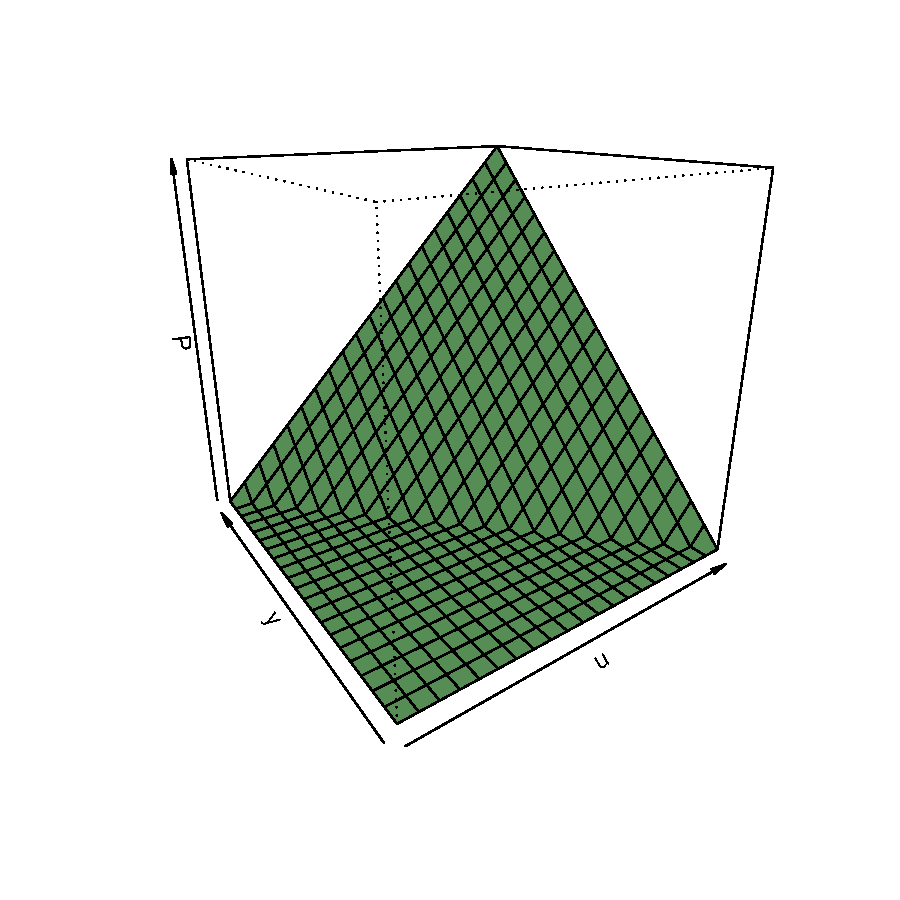
\includegraphics[width = \textwidth]{copulaM.pdf}
    \end{minipage}
    \hspace{.0\linewidth}% Abstand zwischen Bilder
    \begin{minipage}[b]{.3\textwidth} % [b] => Ausrichtung an \caption
      \caption{$\Pi(x, y)$}
      \label{fig:pi}
      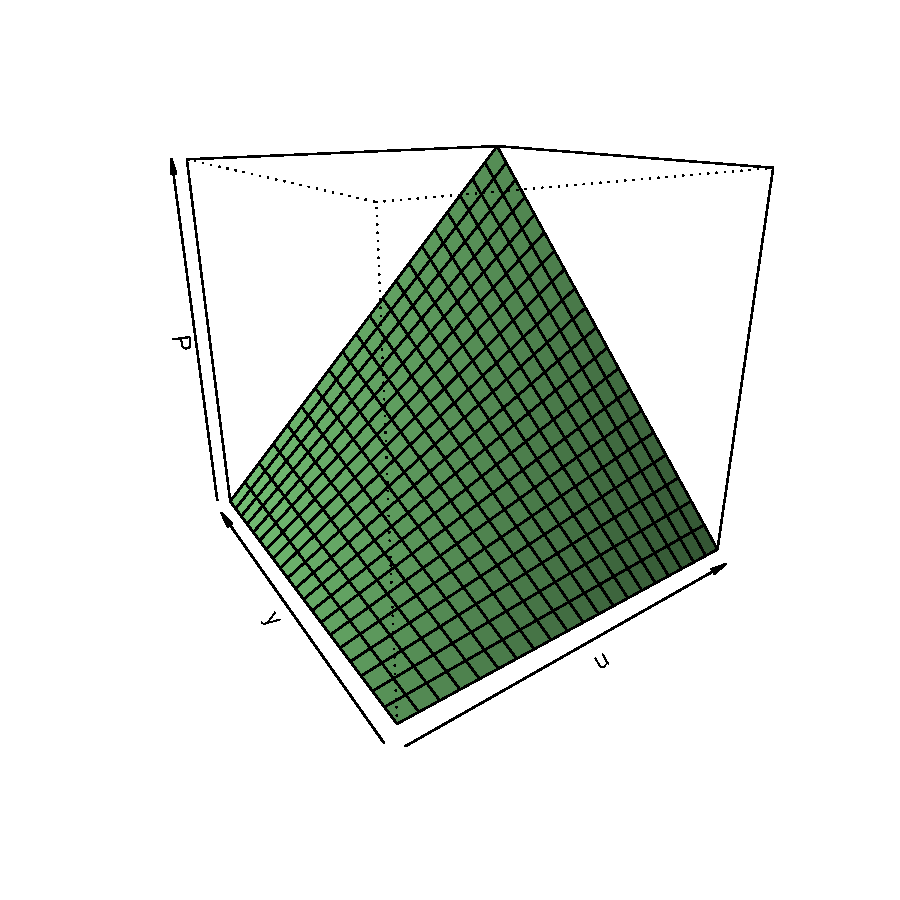
\includegraphics[width = \textwidth]{copulaPi.pdf}
    \end{minipage}
    \hspace{.0\linewidth}% Abstand zwischen Bilder
    \begin{minipage}[b]{.3\textwidth} % [b] => Ausrichtung an \caption
      \caption{$M(x, y)$}
      \label{fig:upper}
      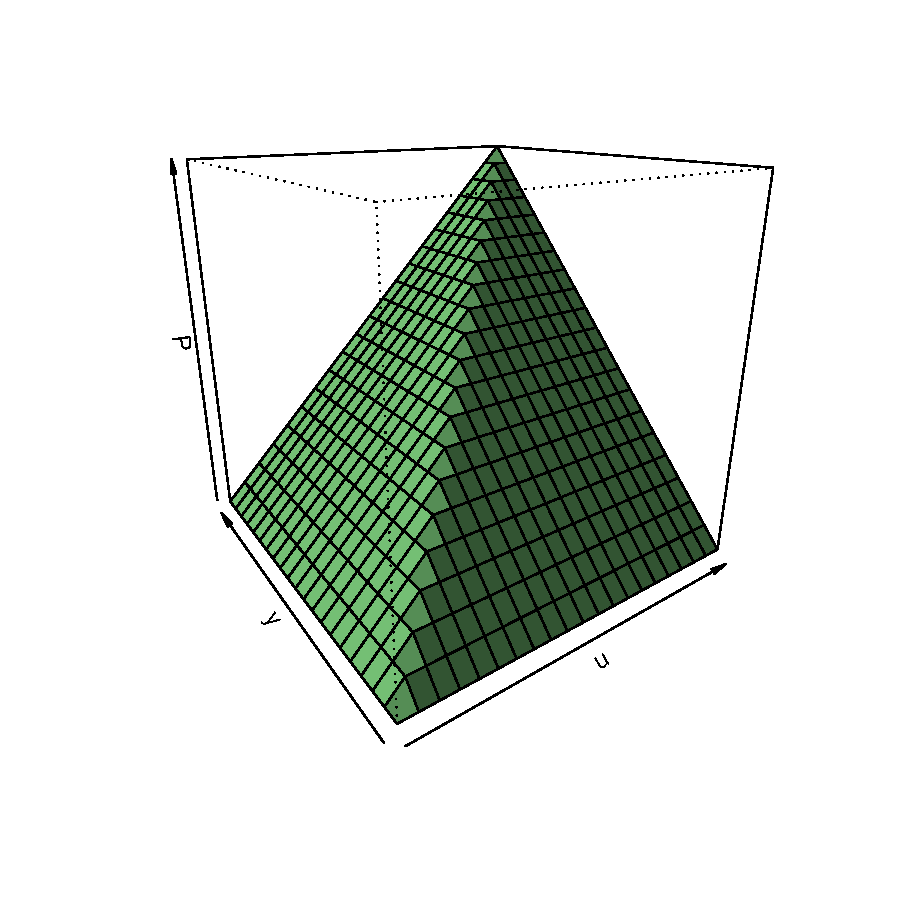
\includegraphics[width = \textwidth]{copulaW.pdf}
    \end{minipage}
  \end{figure}